\documentclass[dvipdfmx,9pt,notheorems]{beamer}
%%%% 和文用 %%%%%
\usepackage{bxdpx-beamer}
\usepackage{pxjahyper}
\usepackage{pdfpcnotes}
\usepackage[absolute,overlay]{textpos}
\usepackage{minijs}%和文用
\renewcommand{\kanjifamilydefault}{\gtdefault}%和文用

%%%% スライドの見た目 %%%%%
\usetheme{metropolis}
\usefonttheme{professionalfonts}
\usecolortheme[RGB={112,128,144}]{structure}
\setbeamertemplate{frametitle}[default][center]
\setbeamertemplate{navigation symbols}{}
\setbeamercovered{transparent}%好みに応じてどうぞ)
\setbeamertemplate{footline}[page number]
\setbeamerfont{footline}{size=\normalsize,series=\bfseries}
\setbeamercolor{footline}{fg=black,bg=black}
%%%%

%%%% 定義環境 %%%%%
\usepackage{amsmath,amssymb}
\usepackage{amsthm}
\theoremstyle{definition}
\newtheorem{theorem}{定理}
\newtheorem{definition}{定義}
\newtheorem{proposition}{命題}
\newtheorem{lemma}{補題}
\newtheorem{corollary}{系}
\newtheorem{conjecture}{予想}
\newtheorem*{remark}{Remark}
\renewcommand{\proofname}{}
%%%%%%%%%

%%%%% フォント基本設定 %%%%%
\usepackage[T1]{fontenc}%8bit フォント
\usepackage{textcomp}%欧文フォントの追加
\usepackage[utf8]{inputenc}%文字コードをUTF-8
\usepackage{otf}%otfパッケージ
\usepackage{sansmathfonts}%数式・英文ローマン体を sansmathfonts にする
\usepackage{bm}%数式太字
%%%%%%%%%%

\title{FreeFlow: Software-based Virtual RDMA Networking for Containerized Clouds}
\author{Daehyeok Kim\footnotemark[1], Tianlong Yu\footnotemark[1], Hongqiang Harry Liu\footnotemark[3], Yibo Zhu\footnotemark[2], Jitu Padhye\footnotemark[2], Shachar Raindel\footnotemark[2], Chuanxiong Guo\footnotemark[4], Vyas Sekar\footnotemark[1], Srinivasan Seshan\footnotemark[1]}
\institute{\footnotemark[1]Carnegie Mellon University, \footnotemark[2]Microsoft, \footnotemark[3]Alibaba, \footnotemark[4]Bytedance}

\begin{document}
\begin{frame}[plain]\frametitle{}
\titlepage %表紙
\end{frame}

\begin{frame}\frametitle{動機}
	\begin{itemize}
		\item 自分が抱えていたタスクの中にRDMAが絡むようなものがあったので知識をつけたかった。
		\item 軽く読んだらもしかして弊社の機械学習とかに提供するインフラとして一考の余地があるのかなと気になった。
		\item 仮想化するのにベアメタル構成と同じくらい性能が出るよと書いてあって、嘘つくなと思った。
	\end{itemize}
	\pnote{
		はじめにこの論文を選んだ動機ですが3つありまして、
		1つ目はRDMAに関する知識をつけたかったという点です。抱えていたタスクにRDMAが少し絡むことがあったのでそれも後押しになっていました。
		2つ目は軽く流し見したときにTensorflowとかをターゲットにしている雰囲気で、もしかしたら弊社の機械学習関係のインフラとして良さそうな感じのものか興味が湧いたからです。
		3つ目は仮想化するのにベアメタル構成と同じくらいパフォーマンス出るよと書いてあって、そんな訳あるかと思ったからです。
		こんな理由から今回はこの論文を取り上げさせてもらいました。
	}
\end{frame}

\begin{frame}\frametitle{Contents}
\raggedright
\tableofcontents
\end{frame}

\section{概要}
\begin{frame}\frametitle{概要}
\begin{itemize}
  \item コンテナを利用した大規模クラウドアプリケーション
  	\begin{itemize}
  		\item high resource efficiency
  		\item	light weight isolation
  	\end{itemize}
	\item その一方でdata-intensiveなアプリケーション(deeplearning, data analytics)は高性能のネットワーク(RDMA)を要求する
	\item コンテナ化によるメリットとRDMAによるメリットをいいとこ取りしたい! $\rightarrow$ \bm{{\color{red} FreeFlow}}
	\item FreeFlowによりベアメタルRDMAと同程度のネットワークパフォーマンスを達成しながらコンテナの恩恵を受けることができる。
\end{itemize}
\pnote{
	まず、本論文の概要をざっくりと説明します。
	近年、大規模クラウド環境でコンテナを利用したアプリケーション開発が盛んにされています。
	コンテナを利用するメリットは大きくて、高リソース効率であることや、軽量な隔離環境でアプリケーションが実行できることなどが挙げられると思います。
	ただし、その一方でデータインテンシブなアプリケーション、例えばディープラーニング関係のものや、データアナリティクス関係のものは、高性能なネットワーク環境、それこそRDMA環境を要求することが多々あります。
	この論文では、コンテナ化によるメリットを享受しながらRDMAによるハイパフォーマンスネットワークを利用する方式として新たにFreeFlowを提唱し、検証によりその性能を確認した、という話です。
}
\end{frame}
\section{目的・背景}
\begin{frame}\frametitle{背景}
\begin{itemize}
  \item コンテナ化のコアメリットは効率的で柔軟なアプリケーションマネジメントの提供である。
	\item containerized cloudではネットワークについて以下の要件をコンテナが満たしていてほしい
	\begin{itemize}
		\item \textit{{\color{red} Isolation}} : containerはそれぞれのnamespaceを持っていてほしい
		\item \textit{{\color{red} Portability}} : virtual networkを利用してどのホストでも固定のvirtual ipでコンテナ間通信できてほしい
		\item \textit{{\color{red} Controllability}} : control / data plane policy をコントロールできてほしい
	\end{itemize}
  \item RDMAの完全仮想化は性能を殺してしまうし、RDMA自体はcontrol / data plane のpolicy変更が難しい
	\begin{itemize}
		\item 実際のところ、TensorFlowやSparkなどは専用ベアメタル + RDMAなどの形態で運用しパフォーマンスを担保するケースがある。
		\item これは提供側にとってもユーザ側にとっても辛い
	\end{itemize}
\end{itemize}
\pnote{
	まず背景からお話します。
	先程話したとおり、コンテナ化には様々なメリットがあり現在ではアプリケーションマネジメントの方式としては非常に復旧しています。
	ここでクラウド環境におけるコンテナの利用を考えたときに、コンテナは以下の要件を満たすことで非常に効率的で柔軟なアプリケーション環境を提供することができると、筆者らは定義付けています。
	1つ目は、ContainerがそれぞれのNetwork namespaceを持っていること。(Isolation)
	2つ目は、virtual networkを利用し、どのホストでも固定のvirtual ipを利用してコンテナ間通信ができること。(Portability)
	3つ目は、コントロールプレーン、データプレーンのポリシーを柔軟にコントロールできること。
	です。

  これらの全てを満たした状態でRDMAの環境を提供することが目的になります。
	ただRDMAの完全仮想化を行えばこれらは達成できそうだけどパフォーマンスが出ないし、逆にRDMAをパススルーする方式をうまくやろうとしてもコントロールプレーンやデータプレーンのポリシー変更が柔軟ではなくなってしまうという問題がある。
	ちなみに現在だと、データインテンシブなアプリケーションは専用ベアメタル+RDMAでパフォーマンスを担保するようなケースが多いようで、この形態は提供側もユーザ側もしんどいよね、という感じ。
}
\end{frame}

\begin{frame}\frametitle{目的}
	\begin{itemize}
		\item \bm{目的} : container環境でもRDMAが使えて、ベアメタル + RDMAくらいの性能が出るようにする!
		\item \textit{Isolation}, \textit{Portability}, \textit{Controllability} に加えて、\textit{high performance} も達成する!
		\item containerから利用できるRDMAのその他の手法に関してまとめたものが下図
	\end{itemize}
  \begin{figure}[htb]
    \centering
    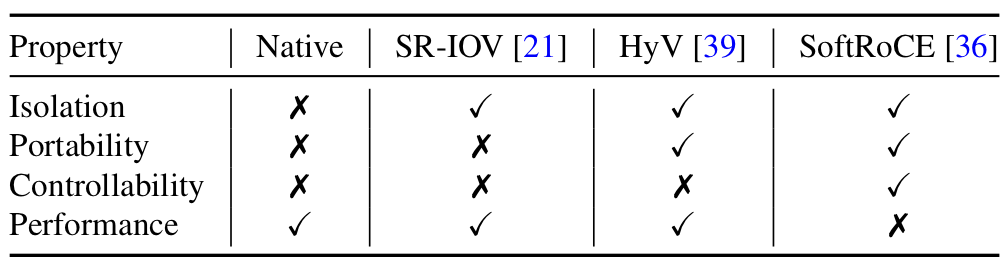
\includegraphics[scale=1]{fig/table1.png}
  \end{figure}%
	\pnote{
		そのため本論文では、先に上げた全てのコンテナ化のメリット+パフォーマンスがベアメタルくらい出るようなRDMA環境をコンテナに提供することが目的です。
	  現時点で存在する、コンテナにRDMA通信を可能にさせる方式と、今回の評価軸にのっとって評価した場合の結果を表にしています。
		* SR-IOVに関しては本質的にPortabilityに難あり。
		* HyVなるものがあるらしい(これは知らないしちゃんと調べられていないが)Visibilityやdata trafficのcontrolができないらしい。
		* SoftRoCEというUDPネットワークスタックの上でRDMAを実行するソリューションは、既存のIPネットワークソリューションを利用して多くを実現できるものの、パフォーマンスはUDPで制限されてしまうため出ない。

    本論文紹介する方式はFreeFlowと読んでいます。以降ではFreeFlowを概要から追って説明していきます。
	}
\end{frame}

\section{FreeFlow}
\begin{frame}\frametitle{FreeFlowの概要}
	\begin{itemize}
		\item RDMAではAPIを利用してアプリケーションからHW NICにコマンドを投げる
		\item FreeFlowではこのアプリケーションとHW NICの間に割って入る。
		\begin{itemize}
			\item FFRでvirtual networkの提供 + control / data plane policyの適用。
			\item FFRは各contianerのmemory領域をshareしていて、App $\rightarrow$ NIC も NIC $\rightarrow$ App もここのメモリを橋渡しにする。
		\end{itemize}
	\end{itemize}
  \begin{figure}[htb]
    \centering
    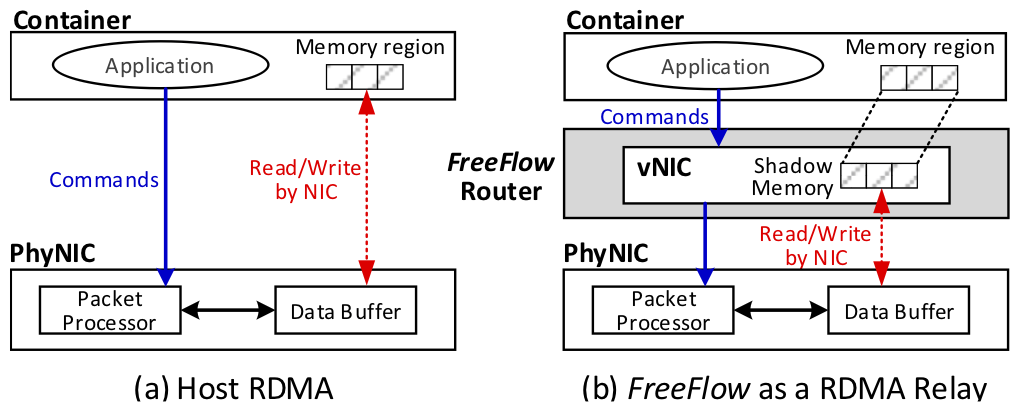
\includegraphics[scale=1]{fig/figure2.png}
  \end{figure}
	\pnote{
		RDMAではAPIを利用してアプリケーションがHW NICに対してコマンドを投げるような形になっています。
		FreeFlowではこのアプリケーションとHW NICの間に一層作る形になります。図でいうとFreeFlow Routerと記述のあるグレーの部分です。
		このFreeFlow Routerでvirtual networkの提供と、コントロールプレーン、データプレーンのポリシーの適用を行います。
		またFreeFlow Routerでは、コンテナのメモリ領域をshareしており、アプリケーションからNICへのデータコピーも、NICからアプリケーションへのデータコピーも、FreeFlow Routerのメモリを橋渡しとする形で行います。
	}
\end{frame}

\begin{frame}\frametitle{Architecture}
	\begin{itemize}
		\item グレーの部分がFreeFlowで修正した部分
  \end{itemize}
  \begin{figure}[htb]
    \centering
    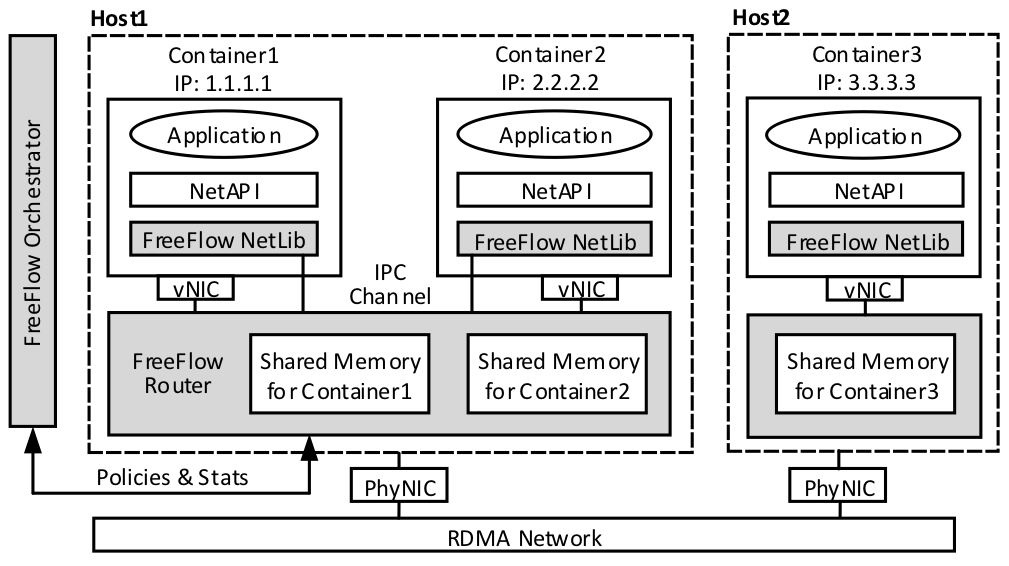
\includegraphics[scale=1]{fig/figure4.png}
  \end{figure}
\pnote{
	全体のアーキテクチャの概要がこちらの図になります。
	これから各部分(FreeFlow Network Library, FreeFlow Router, FreeFlow orchestrator)について説明をしていきます。
}
\end{frame}

% 説明順序変えていいのでは?
\begin{frame}\frametitle{FreeFlow Network Library (FFL)}
	\begin{itemize}
		\item Appコンテナ内部でAppに \\
			    FreeFlow transparentを提供する
		\item ただし、{\color{orange} App内部からは通常のRDMA \\
			    Verbs library を利用しているようにしか見えない}
		\item Appはコードの修正なし \\
			    (もしくはほんの少しの修正)に利用できる
		\item FFRとやり取りする
  \end{itemize}
  \begin{textblock*}{0.4\linewidth} (230pt, 100pt)
  	\centering
		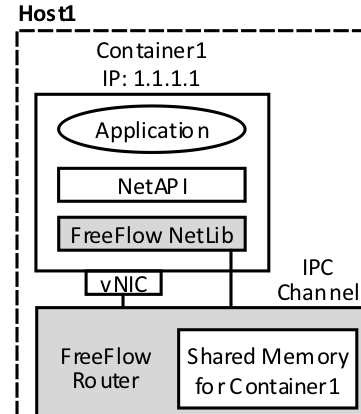
\includegraphics[width=30mm]{fig/figure4-ffl.png}
  \end{textblock*}
\pnote{
	まずはFreeFlow Network Libraryです。
	これはアプリケーションが利用するRDMAのVerbs libraryを改良した感じのものになります。
	ただこれは後ほど説明しますが、Application側が利用するAPIにはほぼ手を付けない形で改良するため、通常のRDMA通信コードから、FreeFlowの通信にするためには、ライブラリの差し替えを行うだけで、アプリケーション側でコードを変更する必要がほとんどないようになっています。
	FFLは次に説明するFreeFlow Routerとやり取りを行います。
}
\end{frame}

\begin{frame}\frametitle{FreeFlow Router (FFR)}
	\begin{itemize}
		\item 各ホストでシングルインスタンス(コンテナ)として起動し、そのホストの各コンテナにvirtual networkの提供を行う
		\item FFLとのchannelをコントロールすることで、data planeのリソースポリシー(QoSなど)を実装する
		\item FFOと連携し、IPアドレスの割り当てなどの処理を行ったりもするらしい。(これはいまいち明記されてなかった)
  \end{itemize}
  \begin{figure}[htb]
    \centering
    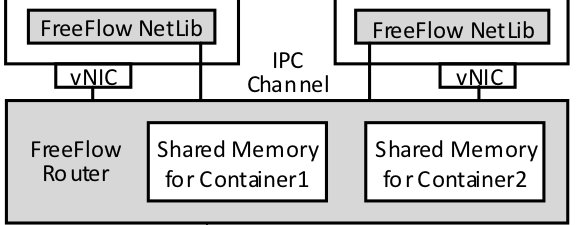
\includegraphics[scale=1]{fig/figure4-ffr.png}
  \end{figure}
	\pnote{
		FreeFlow Routerはホスト毎に一つコンテナで起動し、そのホストに対してvirtual networkの機能提供を行う。
		FFLとのIPC channelをコントロールすることでデータプレーンのリソースポリシーなどを実現します。
		次に説明するFFOを連携することでIPアドレスなどのタスク処理なども行うらしいです。
		FFRが提供するvirtual networkというのがRDMAのみの話ではないのかとも思ったのですが、ちょっと論文の中身では触れられていなかったです。
		ただ実際、Githubの実行例を見ると docker runのタイミングでweaveネットワーク指定できるみたいで、任意のコンテナオーバーレイネットワークソリューションを使用できそうでな形になっていて、TCP/IPで通信をすることもできるみたいなのでそのへんのやり取りのことかなと思っています。
	}
\end{frame}

% ApplicationとFFRのメモリマップの保持だと思うが、これはTransparentの詳細の内容になってしまう。
\begin{frame}\frametitle{FreeFlow Orchestrator (FFO)}
	\begin{itemize}
		\item コントロールプレーンを司る \\
			   (らしいが論文を通してあまり説明が無い。。。)
		\item コンテナ通信のコントロールや \\
			    リアルタイムモニタリングなど。
		\item その他にもユーザ定義情報をストアする。
  \end{itemize}
  \begin{textblock*}{0.4\linewidth} (230pt, 100pt)
  	\centering
  	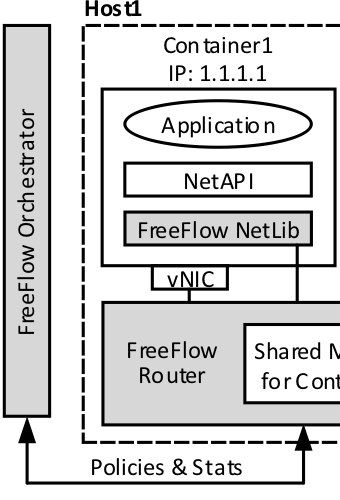
\includegraphics[width=30mm]{fig/figure4-ffo.png}
  \end{textblock*}
	\pnote{
		FFOはコントロールプレーンを司るようなコンポーネントらしいんですが紙面の都合上、FFOの詳細はあまり書いてなかったです。
		コンテナ間通信のコントロールやリアルタイムモニタリングなどを行うようです。
		FFOではZooKeeperを利用してユーザ定義の情報。例えばIPアサインの情報や、アクセスコントロール、リソース共有のポリシー、メモリに関する情報などを管理するそうです。
	}
\end{frame}

% ここの話は性能に関わるのでいる
% RPCの話はまぁしなくていいだろう
\section{Communication channel between FFL and FFR}
\begin{frame}\frametitle{Communication Channel between FFL and FFR}
	\begin{itemize}
		\item FFLとFFRの間のCommunication Channelについて。
		\item FFL側でAppが行ったRDMAリクエスト(APIコール)を、FFR側で模倣する必要がある。
		\item 2つの方式を考えた。
		\begin{itemize}
			\item File Descriptorを利用する。(Unix domain socketによるIPC)
			\item Fastpathを利用する。(Shared memoryによるIPC)
		\end{itemize}
		\item 以降特に断りがない場合、FreeFlowはFastpathによる方式だと思っていただければ。
	\end{itemize}
	\pnote{
		アプリケーションがFFL側で実行したRDMAのAPIコールを、FFR側で実行する必要があります。
		というのも、アプリケーションがコールした内容を、FFR経由でそのホストのPhysical NICに同様のリクエストを必要があるからです。
		つまりあるコンテナから別のコンテナに対してAPI実行をバイパスする必要がある、ということをする。
		直感的に考えつく方法としてRPCがあるかと思います。
		今回は、次に説明する2種類の方法で実現します。
		1つ目は、File Descriptorをうまく変更する方法で、言ってしまえばUnix domain socketによるIPCになります。
		2つ目は、Fastpathという手法で、これはイメージとしてはShared memoryによるIPCになります。
	}
\end{frame}

% Queuenの話が出てきちゃった。。。
\begin{frame}\frametitle{Verbs forwarding via File Descriptor}
	\begin{itemize}
		\item APIコール自体をRPCのように模倣するのではなく、NIC fdに対して行われる要求をFFR側で模倣する。({\color{orange}そのためApp側の変更は少ない})
		\item コンテナ内部のNIC fdをUnix domain socketに差し替える。もう片方の終端をFFRにすることでFFLの内容をFFRに伝える。
		\item Unix Domain SocketベースのIPC
	\end{itemize}
  \begin{figure}[htb]
    \centering
    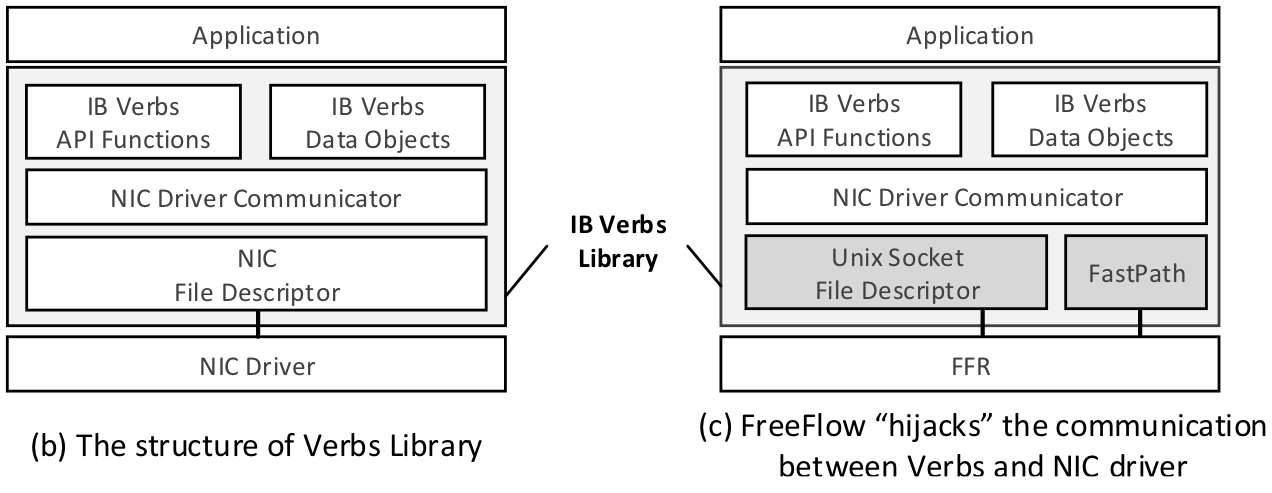
\includegraphics[scale=1]{fig/figure7-bc.png}
  \end{figure}
	\pnote{
		まずはFile Descriptorをうまく変更する方式についてです。
		Verbs Libraryはレイヤ構造になっていて、特にApplication側は結構複雑な構造体のポインタがたくさん出てくる感じになっているので、RPCで行おうとするとかなり深いDeepCopyなどをしないと行けなくて、速度面で問題になってしまいます。
		ただ、NICファイルディスクリプタに対して行われる要求部分は比較的単純になっているらしく、ここをUnix domain socketに差し替え、もう片方の端点をFreeFlow Routerにするようにすれば、FreeFlow Routerに対してNICファイルディスクリプタに対して実行される内容がFFRに伝わることになるので、FFRはそれと同じことをPhysical NICに対して行ってあげる、という手法になります。
		このように、うまくレイヤ構造になっているライブラリの低い部分を差し替えるため、アプリケーション側としては通常のAPIコールをするだけでよいようになっている。
	}
\end{frame}

\begin{frame}\frametitle{File Discriptor方式の欠点}
	\begin{itemize}
		\item レイテンシが大きい。ラウンドトリップタイムを計測したらかんたんに$5\mu$sを超える。
		\item レイテンシセンシティブなアプリケーションでは致命的らしい。
		\item ただし、CPUはほとんど使わない $\rightarrow$ ボトルネックの解消にCPUリソースを少しだけ拝借する設計 \bm{{\color{red} Fastpath}} を考えた
	\end{itemize}
	\pnote{
		ただしこの方式はレイテンシがどうしても大きくなってしまうため、レイテンシセンシティブなアプリケーションではまだ微妙です。
		この方式の良い点はCPUをほとんど利用しない点なのですが、逆にこのボトルネックを解消するためにCPUリソースを少し利用する設計が、次に説明するFastpathになります。
	}
\end{frame}

\begin{frame}\frametitle{Fastpath between FFL and FFR}
	\begin{itemize}
		\item FFLとFFRでメモリを共有する方式。
		\begin{enumerate}
			\item まずFFRがCPUを回し、FFLからのリクエスト、すなわちメモリなにか書かれないか確認する。
			\item リクエストを受け取ったらFFRは直ちに処理する、その際FFLもCPUを回しレスポンスを確認する。
			\item レスポンスが帰ってきたら直ちに処理し、FFL側はCPUを手放す。
	  \end{enumerate}
		\item shared memoryによるIPC
	\end{itemize}
  \begin{figure}[htb]
    \centering
    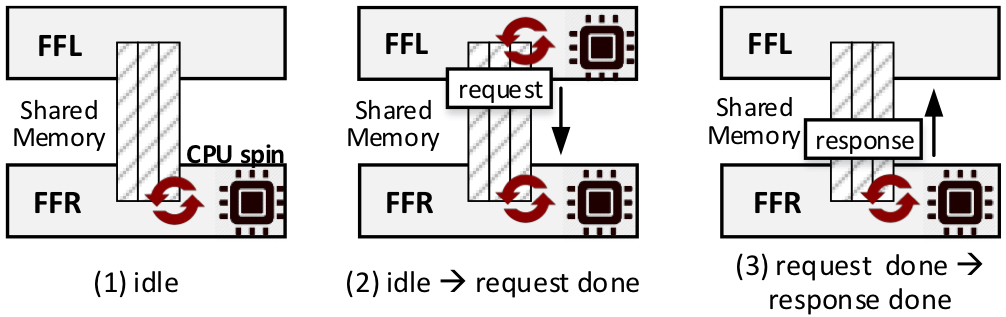
\includegraphics[scale=1]{fig/figure8.png}
  \end{figure}
	\pnote{
		Fastpathは言ってしまえば、shared memoryを利用するIPCになります。
		まずFastpathでは、FFLとFFRでメモリをshareしておきます。
		FFR側ではCPUを(おそらく)pinningし、shared memoryの内容を確認します。
		FFL側ではリクエスト内容をメモリに書き、その内容を受け取った、FFRが直ちにそのリクエスト内容を処理します。
		このタイミングでFFL側でもCPUを利用して、レスポンスを待ち受けます。
		FFRから同様にレスポンス内容がメモリに書かれると、それがFFLに渡り、処理されます。
		FFL側では処理し終わったら、CPUを手放します。
		このようにshared memoryを利用してプロセス間通信をします。
	}
\end{frame}

\begin{frame}\frametitle{Fastpath方式の欠点と対策のための実装}
	\begin{itemize}
		\item CPU を消費する。(メモリチェックが必要)
		\begin{itemize}
			\item 1FFR(つまり1ホスト)で1CPUのみ利用する。複数コンテナの着信確認は1CPUで行うようにデザインした。
			\item non-blockingな関数のときにのみ利用されるなどの制限を設けたため、FFL側でのCPU利用時間は極めて小さい。
		\end{itemize}
		\item FFOはホスト上にレイテンシセンシティブなアプリケーションが無いことを知っている場合、FastpathとCPUの利用を止めることができる。
	\end{itemize}
\pnote{
	Fastpathのメリットはレイテンシが小さいことですが、デメリットはもちろんCPUを消費することです。
	実装的にできる限りCPUの利用を削減するために、いくつか制限を設けているようです。
	1つ目は、1つのFFR、つまり1ホストでは1CPUのみを利用するように、複数コンテナの着信確認を1CPUでおおなうようなデザインにしたということです。
	2つ目は、non-blockingな関数の場合にのみ利用するなどの制限を設け、FFL側でのCPU利用時間は極めて少なくしたということです。
	また、FFOが、ホスト上にレイテンシセンシティブなアプリケーションが存在しないことを確認できる場合はFastpathとCPUの利用を止めるようにできるそうです。
	その判定は、起動しているコンテナの内容で判断すると一言書いてありましたが、詳細はあまりわからなかったです。
}
\end{frame}

\section{Control \& data plane policies}
\begin{frame}\frametitle{Control \& data plane policies}
	\begin{itemize}
		\item FreeFlowではコントロール/データプレーン両方のオペレーションが可能。
		\item 下記のような一般的なコントロール/データプレーンポリシーを適用できる。
		\begin{itemize}
			\item 帯域幅の制御
			\item フローの順位付け
			\item リソース使用の制御
		\end{itemize}
		\item 紙面の都合上、詳細ではないもののcontrol planeの例とdata planeの例を一つづつ挙げてくれている。
	\end{itemize}
	\pnote{
		次にコントロールプレーン、データプレーンのポリシーに関する話です。
		これは論文的にも必要最低限しか書いてなく、「紙面の都合で割愛する」という言葉が結構出てきていました。
		FreeFlowでは基本的にコントロールプレーン/データプレーンの両方のオペレーションが可能で、一般的なポリシーの適用は可能であると記述がありました。
		挙げられていたものとしては、帯域幅の制御や、フローの順位づけ、リソースの制限などです。
		基本的にRDMAはメッセージ単位の通信になるため、そのレベルでの制限はつけられるというような肌感です。
	  コントロールプレーンの例とデータプレーンの例を簡単ですが挙げてくれていました。
	}
\end{frame}

\begin{frame}\frametitle{Control plane policy example}
	\begin{itemize}
		\item 各コンテナが作成できるQP(Queue Pair : RDMA通信において端点に対応するもの)の数に制限をつけることができる。
		\item RDMAにおいて、大量にQPを作成すると性能に影響することが知られている。
		\item コンテナ単位でこのQP数の制御を行うことができる。
	\end{itemize}
	\pnote{
		まずコントロールプレーンのポリシーの例です。
		RDMAにおける通信の端点(TCPとかUDPでいうsocketみたいなもの)にQueue Pairというのがあるんですが、各コンテナが作成できるQPの数に制限をつけることができます。
		一般にRDMAではこのQPの数が膨大になると性能に影響することが知られているようで、これを各アプリケーションが起動するコンテナ単位でリミットを設けてハンドリングすることができます。

		(理論的にQPは一つのHCA(コントローラデバイス)ごとに2^24個作れるものの、メモリの制限で4万〜7万個くらいがせいぜいらしい)
	}
\end{frame}

\begin{frame}\frametitle{Data plane policy example}
	\begin{itemize}
		\item per-flowのレートリミットをかけることができるとのこと。
		\item FFRに簡単なトークンバケットのデータ構造を実装しており
		\begin{enumerate}
			\item アプリケーションがQPを作成したときにFFOにポリシーをチェック
			\item 予め設定されていたレート制限を持つトークンバケットをQPに関連付け
			\item アプリケーションがリクエスト送信要求をするたびにFFRが送信していいかハンドリング
		\end{enumerate}
		\item これはあくまで一例で、実装の仕方は柔軟にできるらしく、APIも提供しているらしいが割愛していた。
	\end{itemize}
	\pnote{
		次にデータプレーンのポリシーの例です。
		フローごとにレートリミットをかけることができるようです。
		FFRの中に簡単なトークンバケットのデータ構造を実装していて
		まず、アプリケーションがQueue Pairを作成したときにFFOにポリシーチェックをし、
		予め設定されていたレート制限を持つトークンバケットをQueue Pairに関連付けて、
		アプリケーションがリクエスト送信要求をするたびに、FFRがトークンバケットを確認し送信するかどうかをハンドリングする
		という流れでレートリミットを実装する形になります。
		ただ、この実装はあくまで今回の論文用の一例らしく、実際にはもっと自由に実装できるようにAPIの提供などを行っているようです。

		このようにして、コントロールプレーンやデータプレーンにポリシーを適用することができます。
	}
\end{frame}


\section{評価}
\begin{frame}\frametitle{構成}
	\begin{enumerate}
		\item Infiniband
		\begin{itemize}
			\item CPU : Intel Xeon E5-2620 2.10GHz 8-core $\times$ 2
			\item RAM : 64GB
			\item NIC : 56Gbps Mellanox FDR CX3
			\item OS  : Ubuntu 14.04 (3.13.0-129-generic)
		\end{itemize}
		\item RoCE
		\begin{itemize}
			\item CPU : Intel Xeon E5-2609 2.40GHz 4-core
			\item RAM : 64GB
			\item NIC : 40Gbps Mellanox CX3 NIC
			\item OS  : Ubuntu 14.04 (4.4.0-31-generic)
		\end{itemize}
	\end{enumerate}
	\pnote{
		評価に利用するサーバー構成としては2種類を整えた。
		1つ目はInfinibandで通信する構成のもの、2つ目はRoCEで通信する構成のものになります。
	}
\end{frame}

\begin{frame}\frametitle{Microbenchmark: Throughput and Latency}
	\begin{itemize}
		\item SEND/WRITEのlatency, bandwidthを測定
		\item ベンチマーク測定用ツールはFreeFlow上で{\color{orange}コードの変更なしに実行できた}
	\end{itemize}
	\pnote{
		RDMAのSEND/WRITEのlatency, bandwidthを測定しました。
		ベンチマーク測定用のツールはFreeFlow上でコードの変更なしに実行できたそうです。
	}
\end{frame}

\begin{frame}\frametitle{Microbenchmark: Throughput}
	\begin{itemize}
		\item 2種類のtestbedでRDMA SEND/WRITEのスループットを測定。
		\item 1GBのデータを2KB〜1MBの単位で分割して転送している。
		\item Host-RDMAはベアメタル + RDMAの性能
		\item message size $\geq$ 8KBの場合、Infiniband/RoCEともにベアメタルの性能と同じになる。
		\item (WRITEのデータはREADよりわずかに良いらしいが論文からは省略されている。)
	\end{itemize}
  \begin{figure}[htb]
    \centering
    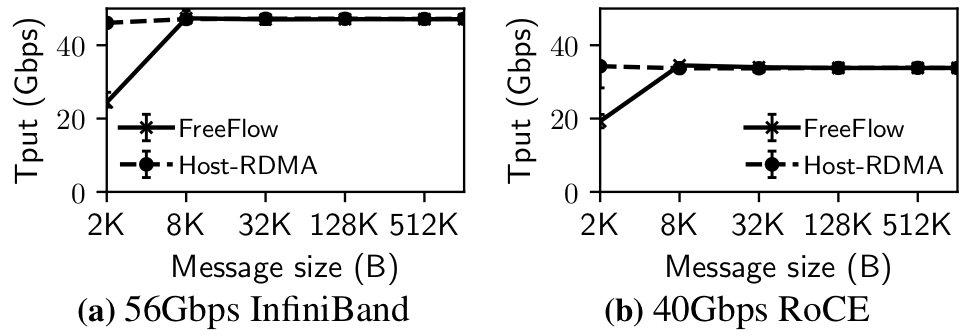
\includegraphics[scale=1]{fig/figure9.png}
  \end{figure}
	\pnote{
		まずはスループットについて、先程述べた2種類の構成で測定したものを、それぞれベアメタル+RDMAの場合と比較した図がこちらの図になります。
		この図は、READの結果ですが、Writeの結果もほぼ同様になったそうで、論文には掲載されていませんでした。
		測定時は1GBのデータを2KBから1MBの単位で分割して転送しています。(横軸)
		メッセージサイズが8KByte以上の場合はInfiniband / RoCEともにベアメタルの性能と同じになっています。
		8KByte未満のところはサイズが細かすぎて帯域が飽和していないだけのようで、実際に2CPUをFFRに利用するとHost-RDMAと同じような値になったようです。
	}
\end{frame}


\begin{frame}\frametitle{Microbenchmark: Throughput}
	\begin{itemize}
			\item 同時稼働コンテナ数(flow数)を512にスケールアップした場合においてもグラフ。
			\item 増加させてもほぼ一定の性能を維持している。(コンテナのスケールにも強い)
			\item このときの帯域幅は各フローで均等に分散していることも確認した。
			\item (このグラフのHost-RDMAは一体なんなのかはよくわからない。。。)
	\end{itemize}
  \begin{figure}[htb]
    \centering
		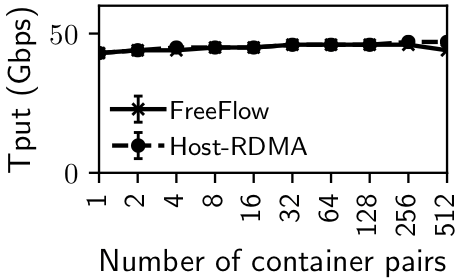
\includegraphics[scale=1]{fig/figure11.png}
  \end{figure}
	\pnote{
		同時稼働するコンテナペア(フロー数)を最大512まで増加させても、全てのフローの集約スループットはほぼ一定の性能を維持していること、及びこのときの帯域幅は各フロードで均等に分さんしていることも測定されました。
		FreeFlowでコンテナを増加させても問題ないことがわかります。
	}
\end{frame}

\begin{frame}\frametitle{Microbenchmark: Latency}
	\begin{itemize}
		\item 64B, 256B, 1KB, 4KBのメッセージを送信し、レイテンシを測定した。
		\item WRITEのほうが、SENDよりレイテンシが少なく、FreeFlowとベアメタルの間のギャップも小さい。
		\item これはFFLとFFRの間のIPCの違いによるレイテンシの差。
		\item とはいえSENDの場合であっても余剰レイテンシは1.5$\mu$s程度。
	\end{itemize}
  \begin{figure}[htb]
    \centering
		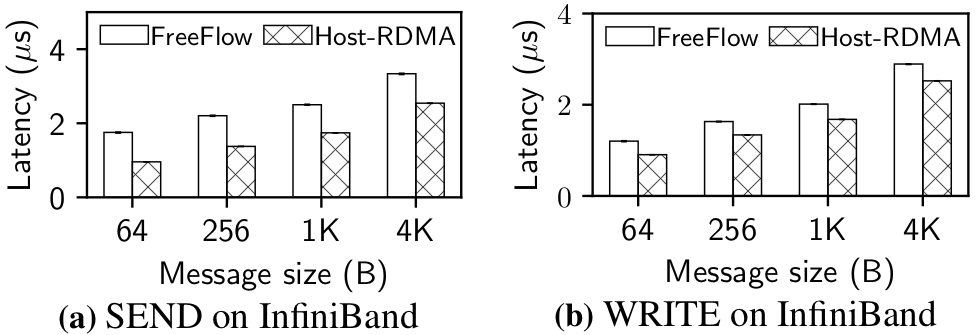
\includegraphics[scale=1]{fig/figure10.png}
  \end{figure}
	\pnote {
		次に、レイテンシについてです。
		こちらはInfinibandの構成で測定しており、64Byte, 256Byte, 1KByte, 4KByteのメッセージ送信のレイテンシを測定しました。
		こちらに関してはWRITEとSENDの両方の結果を掲載していました。
		WRITEのほうがSENDに比べレイテンシが少なっく、FreeFlowとベアメタルのギャップも小さいです。これは今回のスライドでは説明を省いていますが、RDMAの通信方式によりFFLとFFRの間で起こるIPCに違いがあり、その部分のレイテンシが影響しているためです。
		とはいっても、SENDの場合であってもHost-RDMAに比べ余剰のレイテンシは1.5$\mu$s程度です。
		}
\end{frame}

\begin{frame}\frametitle{Microbenchmark: Latency}
	\begin{itemize}
		\item ちなみに、1.5$\mu$sってどれくらい?
		\item ネットワークのone hop : 0.55$\mu$s
		\item TCP stack : least 10$\mu$s
		\item TCP virtual network latency : 40$\mu$s以上(彼らのテストでは)
	\end{itemize}
	\pnote{
		ちなみに1.5$\mu$sってどれくらいかというのも丁寧に書いてくれていました。
		大体、ネットワークのワンホップにかかる時間が0.55$\mu$s程度なので、これが比較対象として上がってくるくらいの速度のようです。
		TCP stackは最低でも10$\mu$s程度、TCP virtual network latencyは40$\mu$s程度にもなるそうなので感覚的喉の程度の速度かはわかっていただけるかと思います。
	}
\end{frame}

\begin{frame}\frametitle{Microbenchmark: CPU overhead}
	\begin{itemize}
		\item Fastpath enableの場合とそうでない場合は実際どのくらいレイテンシに差が出るか。
		\begin{itemize}
			\item Fastpathだと2.4$\mu$sだが、そうでない場合は17.0$\mu$sまで上昇する。
		\end{itemize}
	\item Throughput測定時(このときどのパターンでも帯域はフルに使っており、message sizeは1MB)のCPU UtilizationはやはりLowCPU(disable Fastpath)のほうが断然良い。
	\item {\color{orange}ワークロードによって使い分けるのがベスト}
  \end{itemize}
  \begin{figure}[htb]
  	\centering
		\begin{tabular}{c}
			\begin{minipage}{0.4\hsize}
  			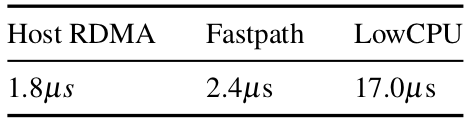
\includegraphics[scale=1]{fig/table3.png}
  		\end{minipage}
			\begin{minipage}{0.4\hsize}
  			\centering
  			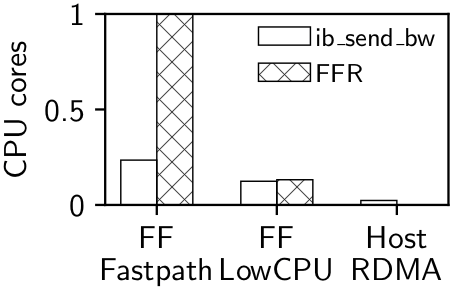
\includegraphics[scale=1]{fig/figure12.png}
  		\end{minipage}
		\end{tabular}
  \end{figure}
	\pnote{
		また、CPUオーバーヘッドに関しても測定しておく。
		Fastpathを用する場合とそうでない場合のレイテンシとCPU coreの利用率を見るとこちらのようになっています。
		まずレイテンシの観点から行くとHost-RDMAが1.8$\mu$sである一方、Fastpathだと2.4$\mu$s、LowCPU(これは名言はなかったですが、おそらくfdを利用する方式)では17.0$\mu$s程度になってしまいます。
		一方で、FastpathはCPUを1つフルに使用しますが、LowCPUでは全然利用しないことがわかります。
	}
\end{frame}

\begin{frame}\frametitle{Microbenchmark: Rate limiter and Performance Isolation}
	\begin{itemize}
		\item rate limiterの性能を検証した
		\item Infinibandのtestbedで、異なるホストのコンテナ間で単一のフローを開始した。
		\item flow rateに制限をかけ、帯域幅を1Gbps〜40GBpsまで変更して測定した。
		\item 複数コンテナペア間でそれぞれに制限をかけても想定通り動いた。
	\end{itemize}
  \begin{figure}[htb]
    \centering
		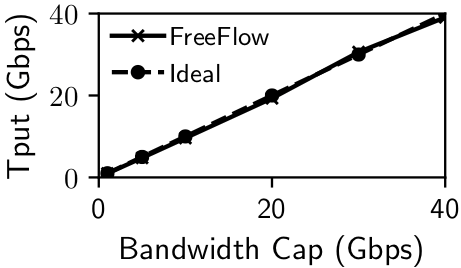
\includegraphics[scale=1]{fig/figure13.png}
  \end{figure}
	\pnote{
		rate limitに関しても検証を行い、データプレーンポリシーがうまく適用されているかの検証も行う。
		frow rateに制限をかけて、帯域幅を変更しながら検証したところ理想的な値を推移することがわかった。
		この実験を、複数コンテナペア間でリミットを変更しながら確認しても問題なく動くことがわかった。
	}
\end{frame}

% 個々らへん理由とかはちゃんと言えるようにする。(書いてある。m)
\begin{frame}\frametitle{Microbenchmark: TCP socket over RDMA}
	\begin{itemize}
		\item 本説とは少しずれる気がするが、socket-based application(rsocket)についても利益をもたらすよという話。
		\item iperfでTCP throughputを、NPtcpを利用してTCP latencyをそれぞれ計測した。({\color{orange}これらも変更の必要はなかった})
		\item Weaveと比べると常に早く、Throughputでホストに勝てないのはsocketとverbsの変換部分のoverhead。
	\end{itemize}
  \begin{figure}[htb]
    \centering
		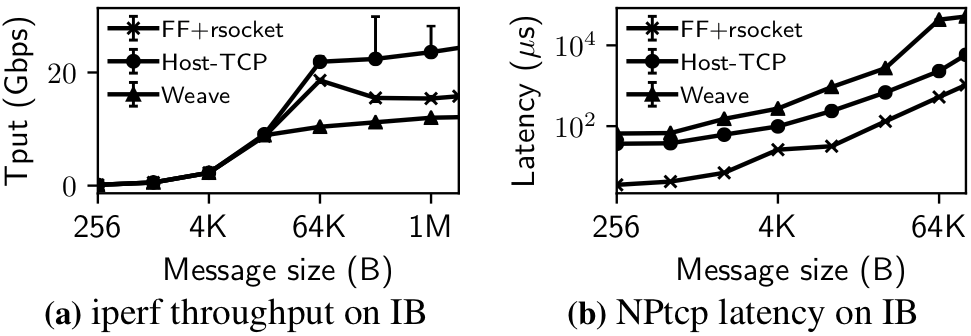
\includegraphics[scale=1]{fig/figure14.png}
  \end{figure}
\pnote{
	rsocket - RDMA socket APIのこと。
	socket-level APIとしてRDMAを提供してくれているプロトコルで、通常のsocket callと同様の取り回しでRDMAを利用できる。
	内部的にはsocketとverbsの変換処理を行っているらしく、Host-TCPほどの性能は出ないものの、Weaveよりは性能が出ている。

	rsocketを利用した性能の検証も行ったようです。
	iperfでTCPのスループット、NPtcpでTCPのレイテンシをそれぞれ計測したところ、virtual nnetworkであるWeaveと比較すると常に早く、Host-TCPには勝てないくらいの性能にはなった。
	Host-TCPに負けている理由はsocketとverbsの間の変換に関するoverheadが原因だということでした。
	}
\end{frame}


\begin{frame}\frametitle{Real-world application}
	\begin{itemize}
		\item TensorflowとSparkを利用して機械学習とデータアナリティクスの性能を確認した。
		\item 比較対象はHost-RDMA(これに近づくほど理想的)、Host-TCP, Weaveの三種類。
		\item これらはすべてInfiniband構成で実行した。
	\end{itemize}
	\pnote{
		ここからは現実的なアプリケーションを取り上げて性能検証の話をしていきます。
		今回はTensorflowとSparkを取り上げ、機械学習とデータ・アナリティクスのアプリケーションの性能を測定しました。
		Infinibandの構成で行い、比較対象はHost-RDMA、Host-TCP、Weaveの三種類です。
	}
\end{frame}

\begin{frame}\frametitle{Tensorflow}
	\begin{itemize}
		\item 3台のサーバ上でRDMA対応のTensorflowを実行。({\color{orange}変更は一行})
		\item 各サーバにはNVIDIA GTX 1080Ti $\times$ 3がそれぞれ搭載されており、一基がmasterかつparameterサーバ, それ以外がworkerサーバ。
		\item 2種類のtraining workloadを実行する
		\begin{itemize}
			\item Convolutional Neural Network : 画像認識用途
			\item Recurrent Neural Network : 音声認識用途
		\end{itemize}
	\end{itemize}
	\pnote{
		まずはtensorflowの性能検証から話します。
		3台のサーバー上でRDMA対応のtensorflowを実行します。
		各サーバにはGPUが搭載されており、一基がmasterかつparameterサーバ、2基がworkerサーバーの構成です。
		training workloadとして、2種類、CNNとRNNを実行しています。
	}
\end{frame}

\begin{frame}\frametitle{Tensorflow: CNN}
	\begin{itemize}
		\item 3種類のモデル(ResNet-50, Inception-v3, AlexNet)をtraining dataとしてImageNet dataを利用。
		\item 分散トレーニングにおいてネットワークパフォーマンスがボトルネックになる。
		\begin{enumerate}
			\item Host-RDMAとHost-TCPの比較をするとRDMAのほうが1.8〜3倍程度良い。
			\item FreeFlowとWeaveを比較するとより大きい差がでている。(Alexnetに関しては14.6倍ほどRDMAのほうが良い)
		\end{enumerate}
		\item FreeFlowの性能はHost-RDMAに切迫している!(Alexnetは少し高いがこれはノイズだろうとのこと)
	\end{itemize}
  \begin{figure}[htb]
    \centering
		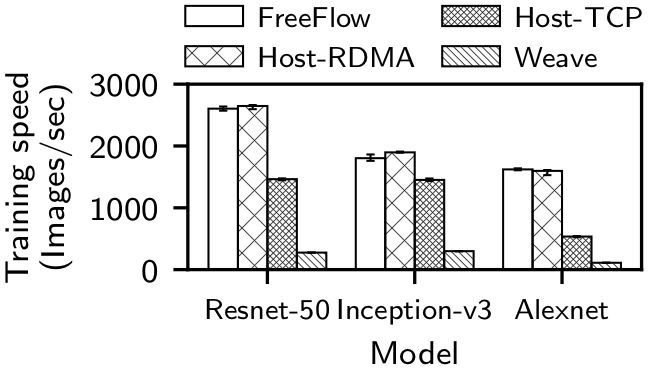
\includegraphics[scale=1]{fig/figure15-a.png}
  \end{figure}
\pnote{
	まずはCNNの方の結果を話します。
	モデルとして利用したのは3種類で、トレーニングデータとしてはImageNetのデータを利用したとのことです。
	分散トレーニングをするわけですが、結果からどのモデルに関しても同じ傾向が見られるため、ネットワークパフォーマンスがボトルネックになっていることがわかります。
	Host-RDMAとHost-TCPを比較するとRDMAのほうが1.8〜3倍程度早いです。
	また、FreeFlowとWeaveを比較すると更に大きい差がでています。
	そのようななか、FreeFlowはHost-RDMAに迫る性能が出ていることがわかります。
}
\end{frame}

\begin{frame}\frametitle{Tensorflow: RNN}
	\begin{itemize}
		\item エンコーダ/デコーダとか隠れ層とかの設定の話があったがちょっと良くわからなかった。。。
		\item 各訓練ステップに費やされた時間をCDFにしたグラフ
		\item CNNの場合と同様に、FreeFlowはHost-RDMAに切迫しており、Weaveに比べて8.7倍くらいの性能が出ている
	\end{itemize}
  \begin{figure}[htb]
    \centering
		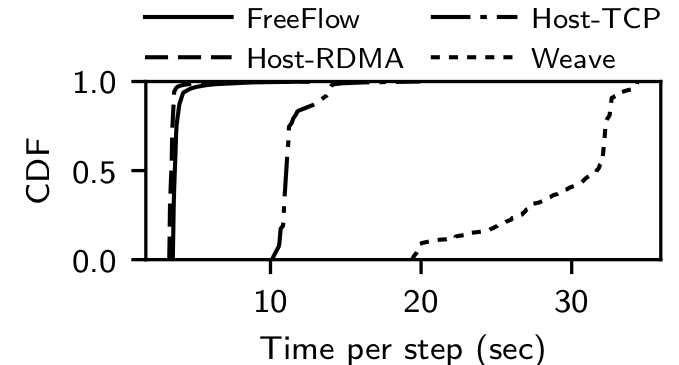
\includegraphics[scale=1]{fig/figure15-b.png}
  \end{figure}
	\pnote{
		次にRNNの方の結果です。
		RNNの設定部分の話はイマイチわかりませんでした。。。
		こちらは各訓練ステップに費やされた時間をCDFグラフにしたものです。
		CNNの場合と同様の傾向を示していて、FreeFlowはHost-RDMAに迫る性能が出ています。
	}
\end{frame}

\begin{frame}\frametitle{Spark}
	\begin{itemize}
		\item 2つのサーバーでSparkを実行。片方にはmaster, slaveのcontainer, もう片方にはslave containerで動作。
		\item Sparkに同梱されている、\textit{GroupBy}と\textit{SortBy}のベンチマークで計測した。
		\item 結果的に、Tensorflowと同様の結果になり、ネットワーク性能がアプリケーション性能に大きく影響しているのがわかる。
		\item FreeFlowはHost-RDMAに切迫しており、Weaveに比べて1.8倍の性能がでる。
	\end{itemize}
  \begin{figure}[htb]
    \centering
		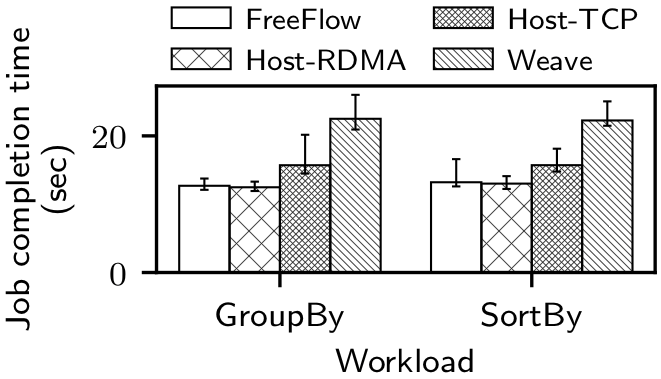
\includegraphics[scale=1]{fig/figure16.png}
  \end{figure}
	\pnote{
		次にSparkの結果について話します。
		こちらは2つのサーバーでSparkを実行し、片方にはmaster, slaveのコンテナ, もう片方にはslaveのコンテナで動作させたそうです。
		Sparkに同梱されているGroupByとSortByというベンチマークで計測したようです。
		結果をみると、こちらもtensorflowと同様の結果になっていることがわかります。
		こちらでもFreeFlowはHost-RDMAに迫る性能が出ていることがわかります。
	}
\end{frame}


\section{Discussion}
\begin{frame}\frametitle{CPU overhead / Congestion Control}
	\begin{itemize}
		\item CPU overhead
		\begin{itemize}
			\item 今回はperformanceためにあえて許容した。
			\item CPUがやるべき仕事をhardwareにオフロードできれば解決は可能かもね。
			\item future workの一つ
		\end{itemize}
		\item Congestion Control
		\begin{itemize}
			\item RDMA NICに輻輳制御メカニズムは入っており、FreeFlowはそれに準拠する。
		\end{itemize}
	\end{itemize}
	\pnote{
		最後にこの方式でいくつか議論になりそうな話に関してまとめて議論しておきます。
		まず、CPUオーバーヘッドについては今回はあえてレイテンシ改善のために許容しました。
		もしうまくハードウェアにオフロードできれば解決はできるかもねという言葉とともに、今後の課題としていました。

		輻輳制御に関してはRDMA NIC側に輻輳制御メカニズムが入っており、FreeFlowはHW NICとしてそれを利用するため、そちらに準拠することになります。
	}
\end{frame}

% TODO: ここは再読
\begin{frame}\frametitle{Security}
	\begin{itemize}
		\item FFRで各コンテナのメモリ状態を取りまとめているから、同一ホストだしIPC領域スキャンすれば確認できるのでは?
		\begin{itemize}
			\item FFRは個々のQPに対して独立して共有メモリバッファを作成するため、IPC領域をスキャンしても他のコンテナの情報は読み取れない.
		\end{itemize}
		\item memory keyの問題(?)。説明がないのでわからなかったが、RDMAの問題なのでFreeFlowで別段悪化はしないらしい。
	\end{itemize}
	\pnote{
		次にセキュリティー的な問題についてです。
		FFRでは各コンテナのメモリを共有するから、IPC領域スキャンすると別のコンテナのメモリ状態見れるのではという問題が考えられますが、FFRでは個々のQueue Pairに対して独立して共有メモリバッファを作成するため、スキャンしても他のコンテナ情報などを読み取ることはできなくなっています。

		また、これは私がわからなかったんですが、memory keyの問題があるよと書いてありました。ただこれに関してはRDMAの問題なのでFreeFlowでどうこうという話ではないよね、とのことでした。
	}
\end{frame}

\begin{frame}\frametitle{Container migration}
	\begin{itemize}
		\item offline migration(shutdown $\rightarrow$ move $\rightarrow$ reboot)可能。
		\item FFR/FFOによりIPアドレスは変わらないので、rebootしたらRDMA connectionを再確立させることができる。
		\item live migrationはできない。
	\end{itemize}
	\pnote{
		コンテナマイグレーションに関しては、まずオフラインマイグレーション、すなわちシャットダウンして、移動して、再起動する形のマイグレーションに関しては可能で、virtual IP が変わらないのでそのままRDMAの接続を再確立するそうです。
		(これはRoCEみたいなIP層を利用するものだとわかりますが、InfinibandだとそもそもIP使うっけ?みたいなレベルの理解が無いのでちょっとわかりません。)
		ただしライブマイグレーションはできないということでした。
	}
\end{frame}

\begin{frame}\frametitle{VM host / Work with external legacy peer}
	\begin{itemize}
		\item VM上でコンテナを動作させる場合
		\begin{itemize}
			\item 今回のprototypeでは基本的にベアメタル上にコンテナを起動させているが、SR-IOVなどを利用しているVM上なら可能。
		\end{itemize}
		\item その他RDMAピアとの通信
		\begin{itemize}
			\item FFRはリモートのpeerがFFR使ってるか普通のRDMAかなどの判別をするわけではないため、RDMAで普通に通信可能。
		\end{itemize}
	\end{itemize}
	\pnote{
		VM上でコンテナを起動させる場合にFreeFlowが使えるのかという問題に関しては、今回のプロトタイプでは基本的にコンテナはベアメタル上で動かしていたが、SR-IOVなどを利用しているVMであれば問題ないだろうと書いてありました。
		その他のRDMAピアとの通信はどうなるのかという問題は、基本的に通信対象がFRRを利用しているかどうかなどは関係しないため、RDMAで普通に通信することが可能になっているということでした。
	}
\end{frame}


\section{結論}
\begin{frame}\frametitle{結論}
	\begin{itemize}
    \item FreeFlowにより、コンテナ環境に対して、\textit{Isolation}、\textit{Portability}、\textit{Controllability}、\textit{Performance}を満たすRDMA環境を提供することができた。
  	\item 肝心のPerformanceに関してもベアメタルRDMAに匹敵するくらいの性能が出る。
		\item Githubは\href{https://github.com/microsoft/Freeflow}{こちら}
	\end{itemize}
	\pnote{
		結論です。
		FreeFlowによりコンテナの環境に対して、Isolation, Portability, Controllability, Performanceを満たすRDMA環境を提供することができるようになりました。
		Controllabilityに関してはmicrobenchmarkでうまくフロー制御ができていることがわかりました。
		肝心のPerformanceに関してもベアメタルRDMAに匹敵するくらいの性能が出ることをいくつかの性能検証で確認できました。
		一応Githubで公開してくれていて、まだプロトタイプ段階とのことですが、ハードウェア要件を満たせば試して確認することもできると思います。issueを見ると、k8sへの対応なども勧めていて、結構頑張っていそうだなという印象でした。
		以上で、発表は終わりです。何か質問等あればいただければと思います。
    論文の内容を省いている部分もあるので、話していない論文の内容についても何かあれば質問いただければと思います。
	}
\end{frame}

\newcounter{finalframe}
\setcounter{finalframe}{\value{framenumber}}
\setcounter{framenumber}{\value{finalframe}}
\end{document}
